\documentclass{sig-alt-release2}
% \documentclass{sig-alternate}

\usepackage{amssymb}
\setcounter{tocdepth}{3}
\usepackage{graphicx}
\usepackage{url}
\usepackage{subfigure}

%%%%%%%%%%%Añadido de CPB para controlar las versiones%%%%%%%
%Macros par los cambios
\usepackage[usenames]{color}
%\usepackage[dvips]{color}
\usepackage{colordvi}
\usepackage{ulem}
\normalem
\balancecolumns
%%%%%%%%%%%%%%%%%%%%%%%%%%%%%%%%%%%%%%%%%%%%%%%%%%%%%%%%%%%%%%%%


\begin{document}
\conferenceinfo{GECCO'11,} {July 12--16, 2011, Dublin, Ireland.} 
\CopyrightYear{2011} 
\crdata{978-1-4503-0690-4/11/07} 
\clubpenalty=10000 
\widowpenalty = 10000
\title{Intrinsic Evolvable Hardware for Combinatorial Synthesis Based on SoC+FPGA and GPU Platforms}
\numberofauthors{4}
\author{
\alignauthor
Carlos Camargo Bare�o\\
       \affaddr{Universidad Nacional}\\
%        \affaddr{Bogot�, Colombia}\\
       \email{cicamargoba@unal.edu.co}
\alignauthor
Cesar Pedraza Bonilla\\
       \affaddr{Universidad Santo Tom�s}\\
%        \affaddr{Bogot�, Colombia}\\
       \email{cesarpedraza@usantotomas.edu.co}
\and
\alignauthor
Luis Fernando Ni�o \\
       \affaddr{Universidad Nacional}\\
%        \affaddr{Bogot�, Colombia}\\
       \email{lfninov@unal.edu.co }
\alignauthor
Jose Martinez Torre\\
       \affaddr{Universidad Rey Juan Carlos}\\
%        \affaddr{Madrid, Espa�a}\\
       \email{joseignacio.martinez@urjc.es}
}
\maketitle
\begin{abstract}
This paper presents a novel a parallel genetic programming (PGP) boolean synthesis implementation on a low cost cluster of an embedded open platform called SIE. Some tasks of the PGP have been accelerated through a hardware coprocessor called FCU, that allows to evaluate individuals onchip as intrinsic evolution. Results have been compared with GPU and HPC implementations, resulting in speedup values up to approximately 2 and 180 respectively. 
\end{abstract}

% A category with the (minimum) three required fields
\category{B.5.2}{Hardware}{R-T-L implementation}[optimization]

\terms{Design, Performance}

\keywords{Hardware copyleft, Evolutionary, boolean synthesis}

\section{Introduction}

As an alternative to the traditional design of combinatorial circuits, some authors have proposed bio-inspired techniques to create combinatorial circuits that can not be obtained with the traditional methods and to add some restrictions to the design such as delay, area, etcetc, \cite{Kajitani:1996p16, Aguirre:2009p66, coello2000}. One of the main problems to create circuits by using these techniques is the response time, due the high computational requirements. In order to use parallel genetic programming (PGP), an FPGA cluster-based architecture to solve the combinatorial synthesis problem on-chip has been developed. The fitness coprocessor unit (FCU) on each FPGA helps to accelerate the convergence of the algorithm, as well as provide an appropriate support for 12-variable synthesis problems. The success of the system is mainly due to the capability of evaluating a chromosome in the FPGA through a virtual LUT-oriented architecture without using partial reconfiguration techniques, and determining the fitness value for an individual faster than other related works. 
The copyleft hardware project SIE \cite{CC11b} \cite{CC11d} created by our team work, is composed of a custom embeddded platform and a software development kit based on Linux operating system; allowing the generation of commercial applications under the Creative Commons BY-SA licenses, which allows the distribution and modificacion of the design.

\section{GP Implementation} 
\textbf{HPC and SIE:} The GP was implemented in SIE, a Graphics Processing Unit (GPU) and on ALTAMIRA (High Performance Computer). The GP was implemented in two stages: the first one is about software development and its parallelization on HPC and GPUs, and the second one refers to a hardware implementation to speed it up on the SIE plataform. Using the island approach, the population is divided into sub-populations that will evolve in each processor of the cluster or parallel architecture, making data migration to accelerate convergence. 

\textbf{GPU: } In the GPU platform a function called $kernel-GP$ is executed on each processing element that evolves a sub-population of the GP. Additionally, a  Mersenne-twister algorithm is executed on the GPU before the $kernel-GP$ to make a buffer of random numbers on its own global memory. A thread $t$ generates a $\mu$-population, performs the GP operators during $P$ generations required. $M$ best individuals will be transferred to the global memory and then to the host device (CPU system).

A profiling determined that the most costs were the fitness function calculation and the new individual generation. They have been accelerated with a dedicated hardware in the FPGA (FCU). Inside (figure \ref{fig:hw_block}), the chromosome cells are converted to an equivalent Virtual Look Up Table (VLUT) with a ROM based translation, in order to calculate of wrong minterms compared to the objective function. Also, the FCU calculates the final fitness value including the number of gates and the critical path. In order to speed up pseudo random number generation, a Mersenne-Twister-based coprocessor was inserted through the same custom interface. 

\begin{figure}[htpb]
\begin{center} 
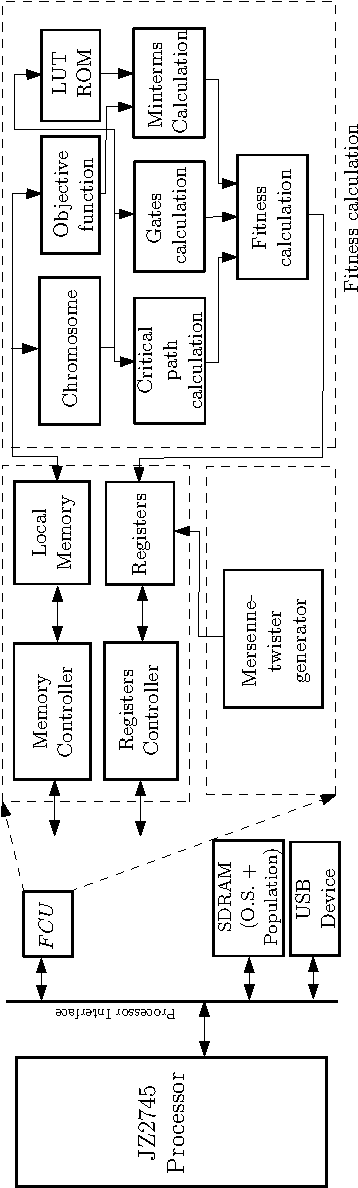
\includegraphics[scale=.42, angle=270]{./images/hw_block_diagram} \end{center}
\caption{FCU structure.}\label{fig:hw_block}
\end{figure}

\section{Performance evaluation.}
SIE performance was compared to HPC (512 processors) and GPU (192 CUDA cores). The response time is measured in three scenarios: 1) number of input variables corresponding to a comparator problem of 2, 4 and 6 bits; 2) population size and 3) number of nodes running the experiment, ranged from 1 to 6 in SIE, and 2 to 16 or 64 in ALTAMIRA. The first and second parameters determine the size of the problem. 

\textbf{Response Time:} Figure \ref{fig:rt_vars} shows the response time for both platforms with different numbers of nodes and variables with 1024 individuals during 100 generations. These results show the high performance of SIE cluster. This experiment demonstrates that the response time for SIE does not depend on the size of the problem. In contrast, response time in ALTAMIRA has a high dependency of the size of the problem, because individuals had to be evaluated by software. Figure \ref{fig:rt_indv} shows the response time in both architectures when varying the number of individuals of the population. It is observed that both architectures have a strong dependency of the number of individuals. This is because increasing this number causes an increment of the software computational load for both clusters. Even in this scenario, SIE shows an excellent performance compared to ALTAMIRA. Figure \ref{fig:rt_indv2} shows the response time of executing the GP in the graphics hardware with problems of 4, 8 and 12 variables. Varying the number of islands and threads, can be observed that the best scenario is obtained when the number of threads is increased independently the number of islands. This is because when more threads are launched more parallelism is performed in the system, until the maximum of threads permitted by the GPUs is reached. The speedup of the SIE vs ALTAMIRA was up to 180 for 12-variable problems. The excellent performance of SIE can be explained because individuals have been directly tested in hardware (FPGA), obtaining a combination of their true table on each cycle of the system clock. On the other hand, individuals evaluated in software by ALTAMIRA require a lot of system clocks, causing response times hundreds of times higher than SIE. On the other hand, the speedup number when SIE and GPU are compared was up to 2 for 12-variable problems. This can be explained because the whole population have been tested in hardware, obtaining a combination of their output on each cycle of the system clock. But, when an individual is tested in software, each combination requires a set of instructions, that requires a lot of cycles of the system clock.
  \begin{figure}[h!]
    \begin{center}
      \subfigure[SIE vs ALTAMIRA.]{
        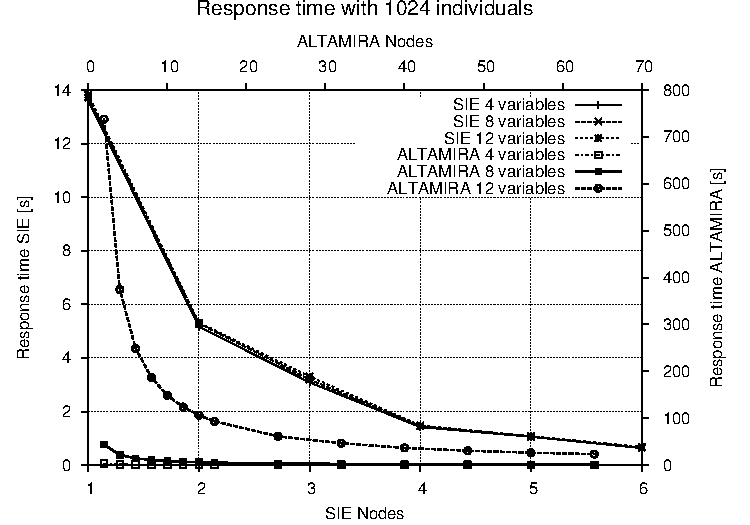
\includegraphics[width=6cm, height=3cm]{./images/response_time_1024indiv} 
        \label{fig:rt_vars}
      }
      \subfigure[SIE vs ALTAMIRA.]{
        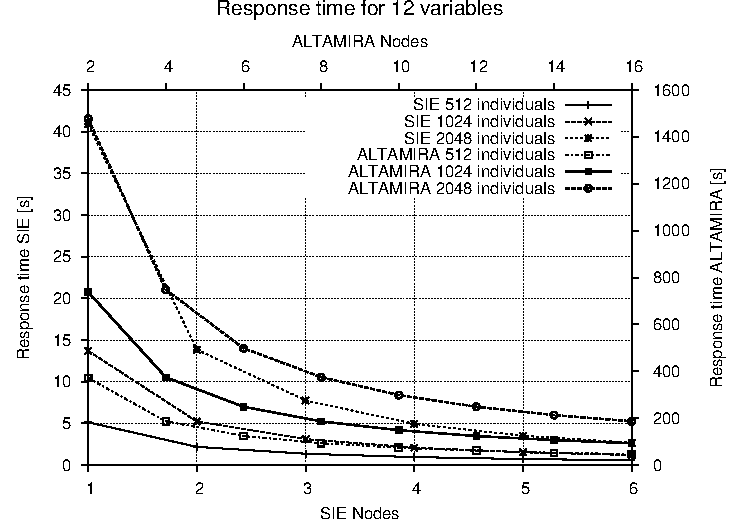
\includegraphics[width=6cm, height=3cm]{./images/response_time_12var} 
        \label{fig:rt_indv}
      }
      \subfigure[SIE vs GPU.]{
        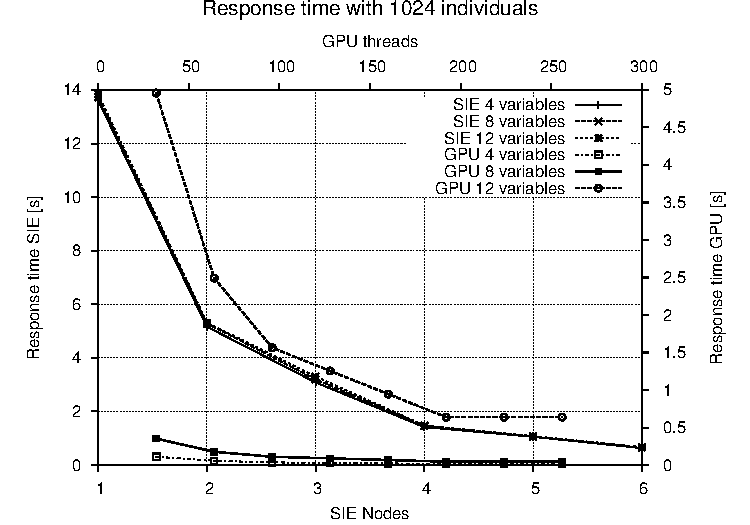
\includegraphics[width=6cm, height=3cm]{./images/response_time_1024indiv_gpu}  
        \label{fig:rt_indv2}
      }    \end{center}
   \caption{Response time comparison SIE, ALTAMIRA, GPU}
  \end{figure}
% &&&&&&&&&&&&&&&&&&&&&&&&&&&&&&&&&&&&&&&&&&&&&&&&&&&&&&&&&&&&&&&&&&&&&&&&&&&&&&&&&&&&&&&&&&&&&&&&&&&&
%                                                                     CONCLUSIONES Y TRABAJO FUTURO
% &&&&&&&&&&&&&&&&&&&&&&&&&&&&&&&&&&&&&&&&&&&&&&&&&&&&&&&&&&&&&&&&&&&&&&&&&&&&&&&&&&&&&&&&&&&&&&&&&&&&
\section{Conclusions and future work.}
This paper presented a novel way to evaluate individuals in an intrinsic evolvable algorithm on an open embedded platform, and results were compared to an HPC called ALTAMIRA and a high performance NVIDIA GPU. To accelerate the evolution process, a coprocessor was implemented to calculate the fitness function and to generate random numbers, improving the performance for problems with more than 6 bits. Results showed a speedup of 2 when SIE was compared to GPU (192 processors). When compared with ALTAMIRA, SIE showed a speedup up to 180; significant speedup were obtained due individuals have been directly tested in hardware.
Tests proved that the algorithm is more effective for 4-bit and 8-bit problems. 12-bit problems in SIE had excellent performance, but because the search space is too long, converging to a suitable solution was difficult for the algorithm. This problem could be solved as future work with some improvements in terms of multiple FCUs inside an FPGA, more nodes, and other hardware-accelerated genetic operators.
\bibliographystyle{plain}
\bibliography{./biblio_EHW.bib}
\end{document}
